\documentclass[]{article}
\usepackage{graphicx}
\usepackage[margin=1cm]{geometry}
\usepackage{csvsimple}
\usepackage{hyperref}

\begin{document}
\listoffigures
\listoftables

\newpage
\section*{\centering $ 0.3 < p_T < 1.5$ and $ |\eta|<1$}
\subsubsection*{\centering All NPOMS and NPOMH=0}

\begin{figure}[h!]
    \centering
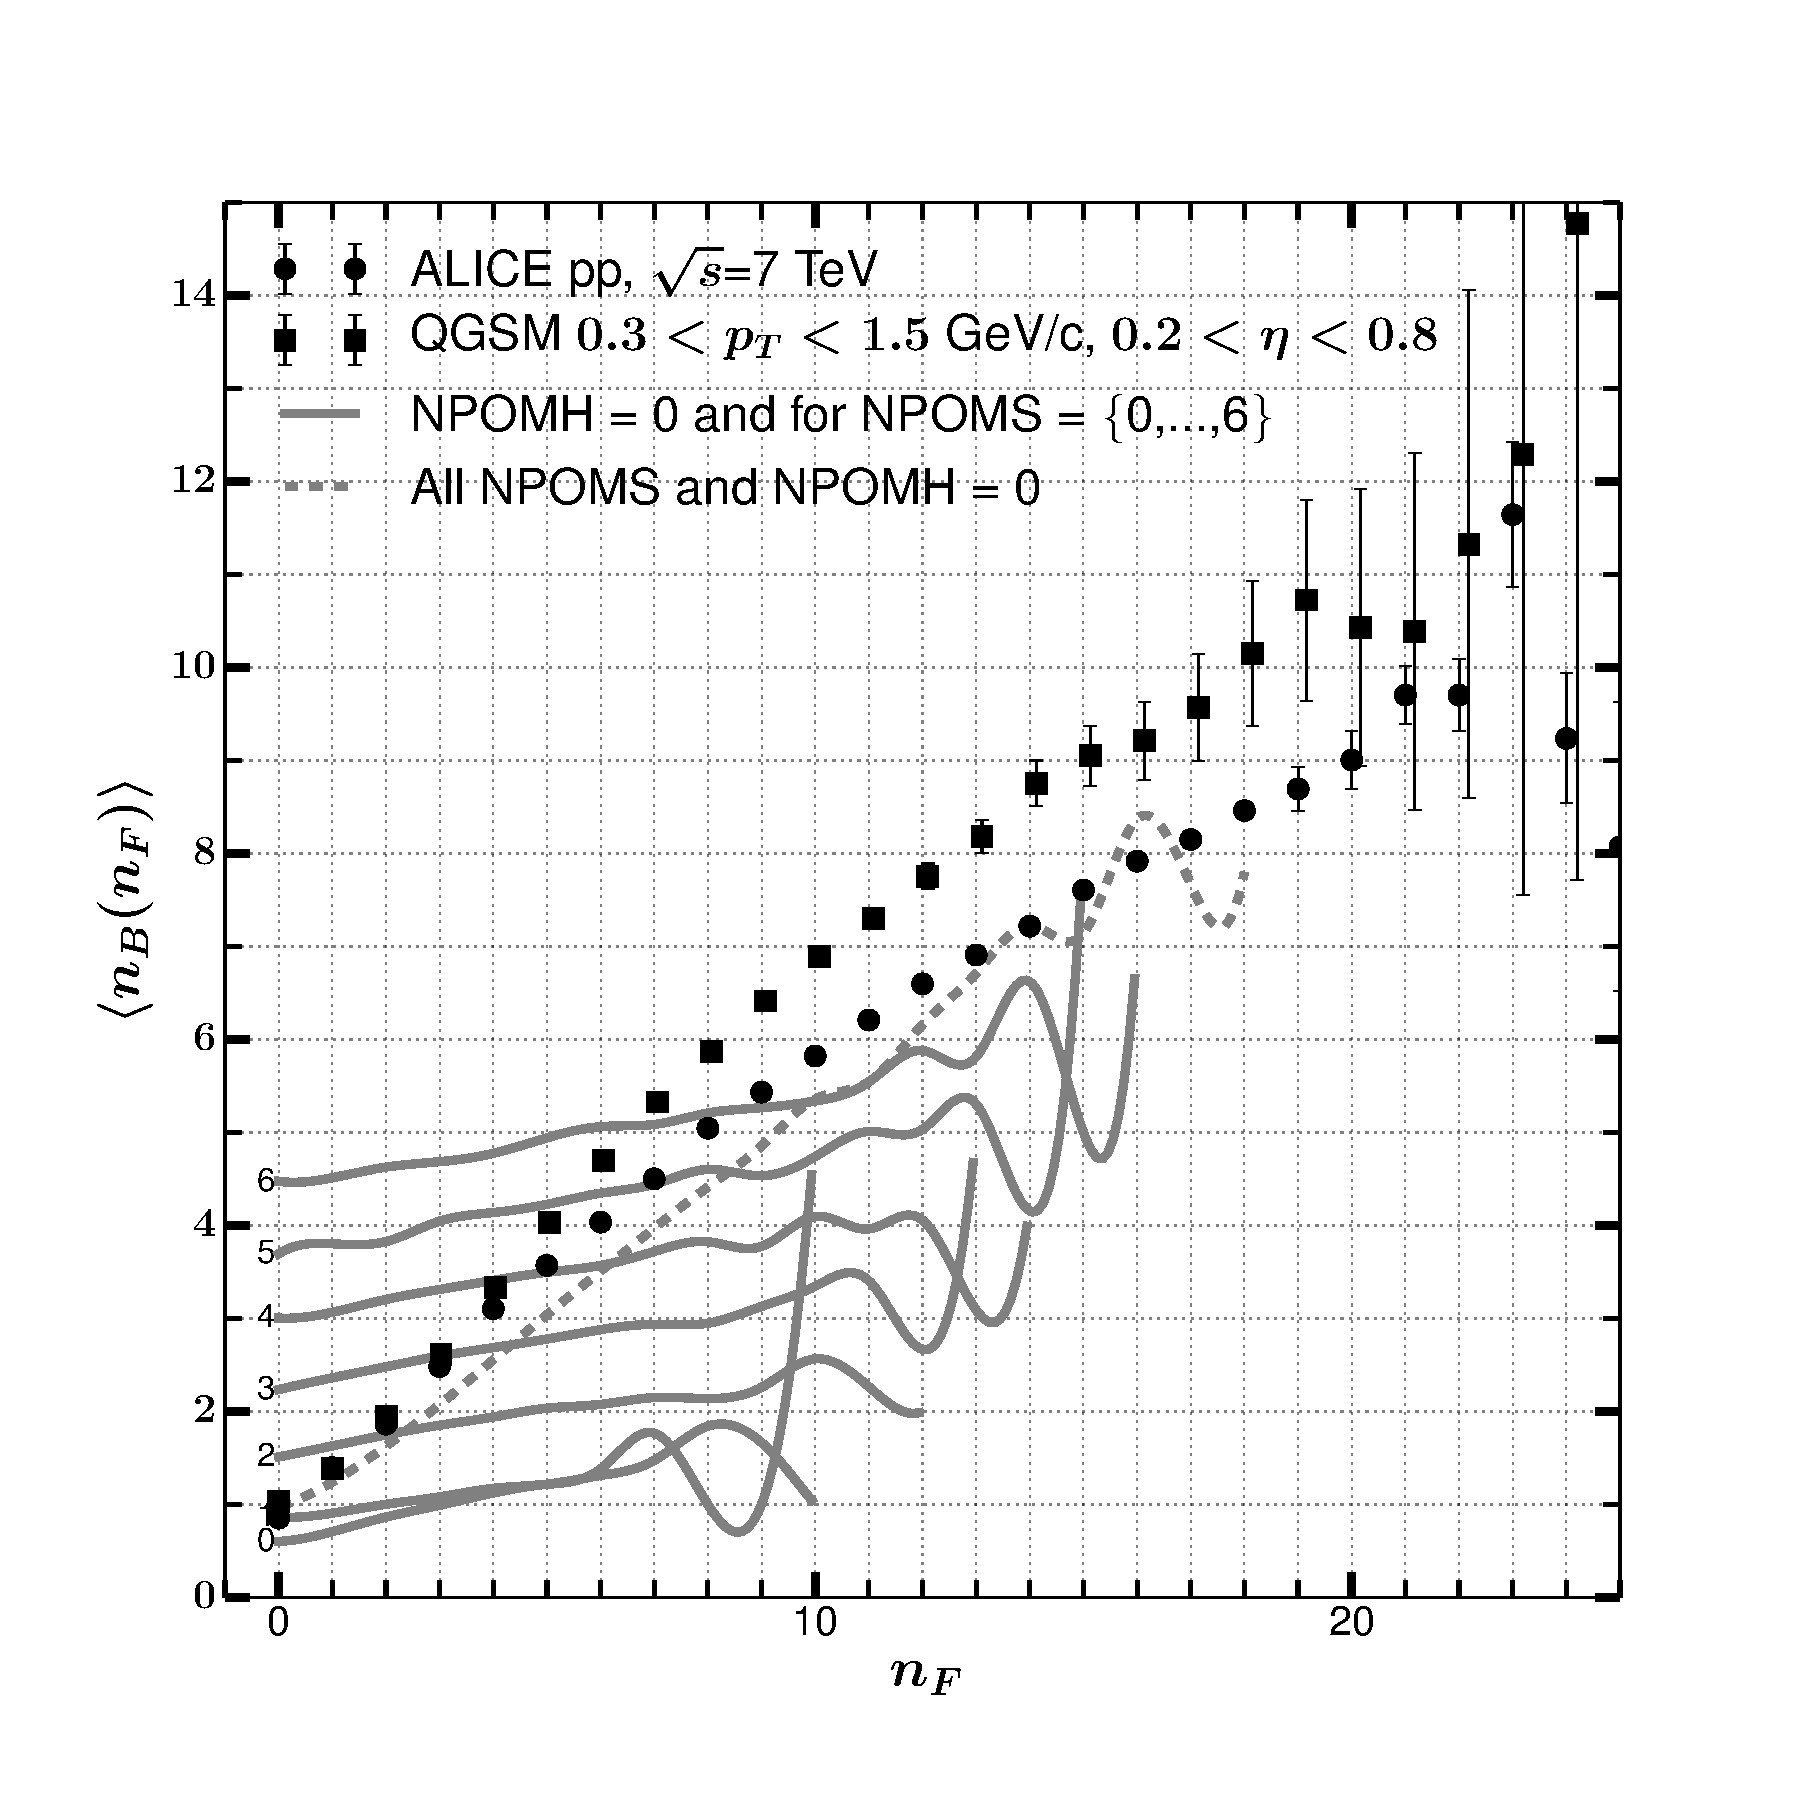
\includegraphics[scale=0.5]{../analyzed/nbnf_allnpoms_0npomh.pdf}
    \caption[All NPOMS and NPOMH=0]{}
\end{figure}

\begin{table}[h!]
\centering
    \begin{tabular}{|l|l|l|c|l|l|l|l|}
        \hline
Label     & a      & b     &     & $\eta_{gap}$ & $\delta\eta$ &Exp. $b_{corr}$ &Sim. $b_{corr}$\\\hline
Exp. fit  &$0.9175\pm0.000000$&$0.5551\pm0.000000$&  & 0.0 		    & 0.2 		   &$0.366 \pm0.009$&0.360\\\hline
All NPOMS &$0.9609\pm0.002077$&$0.5503\pm0.001395$&	 & 0.2 			& 0.2 		   &$0.358 \pm0.008$&0.358\\\hline 
$N = 8$	  &$0.9700\pm0.002078$&$0.5326\pm0.001397$&	 & 0.4 			& 0.2 		   &$0.345 \pm0.008$&0.353\\\hline
$N = 7$	  &$0.9761\pm0.002079$&$0.5174\pm0.001401$&	 & 0.6 			& 0.2 		   &$0.334 \pm0.008$&0.348\\\hline
$N = 6$	  &$0.9836\pm0.00208 $&$0.4928\pm0.001409$&	 & 0.8 			& 0.2 		   &$0.327 \pm0.008$&0.343\\\hline
$N = 5$	  &$0.9911\pm0.002078$&$0.4542\pm0.001421$&	 & 1.0 			& 0.2 		   &$0.316 \pm0.006$&0.337\\\hline
$N = 4$	  &$0.9928\pm0.002066$&$0.3983\pm0.00144 $&	 & 1.2 			& 0.2 		   &$0.311 \pm0.009$&0.334\\\hline
$N = 3$	  &$0.9775\pm0.002036$&$0.3225\pm0.001471$&	 & 0.0 			& 0.4 		   &$0.521 \pm0.010$&0.524\\\hline
$N = 2$	  &$0.9249\pm0.001978$&$0.2266\pm0.001527$&	 & 0.4 			& 0.4 		   &$0.487 \pm0.012$&0.511\\\hline
$N = 1$	  &$0.7992\pm0.001934$&$0.1156\pm0.001678$&	 & 0.8 			& 0.4 		   &$0.463 \pm0.014$&0.496\\\hline
          &	                  &               &	     & 0.0			& 0.6		   &$0.598 \pm0.011$&0.615\\\hline
	      &                   &               &      & 0.4 			& 0.6 		   &$0.564 \pm0.012$&0.597\\\hline
		  &	                  &               &	     & 0.0 			& 0.8 		   &$0.643 \pm0.011$&0.669\\\hline
    \end{tabular}
\caption[b correlation table]{}
\end{table}

\newpage
\subsubsection*{\centering N NPOMS and all NPOMH}

\begin{figure}[h!]
\centering
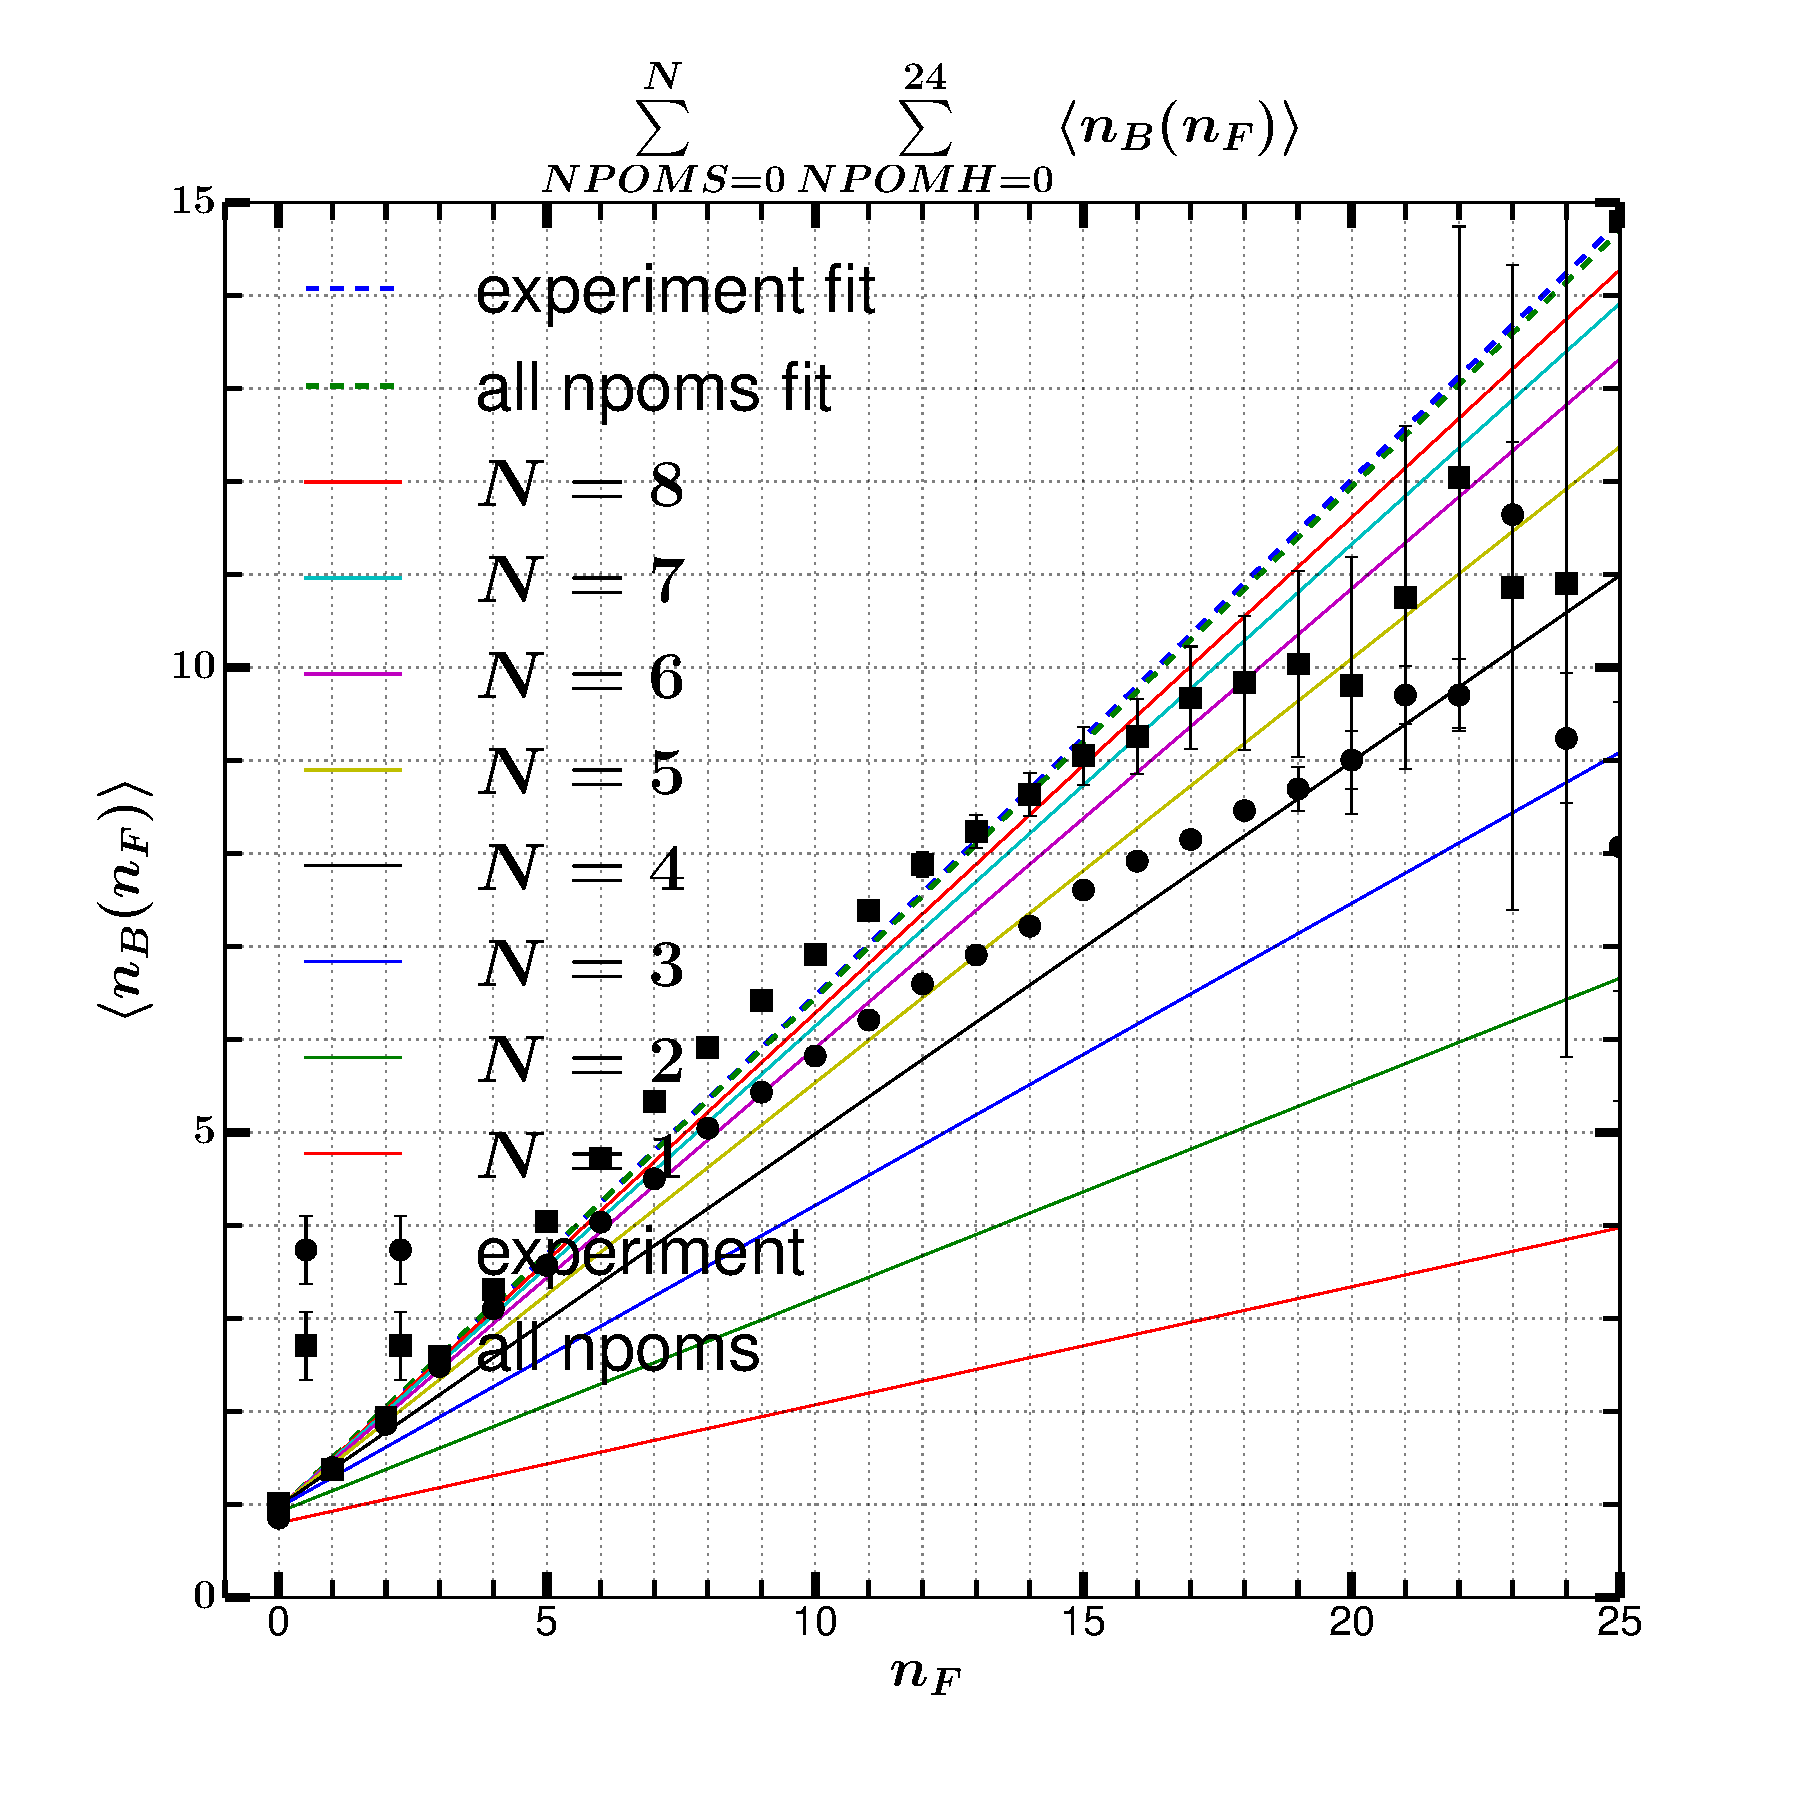
\includegraphics[scale=0.5]{../analyzed/nbnf_Nnpoms_allnpomh.pdf}
    \label{fig1}
    \caption[N NPOMS and all NPOMH]{}
\end{figure}

\newpage
\subsubsection*{\centering Fixed NPOMS and varying NPOMH}

\begin{figure}[h!]
    \centering
    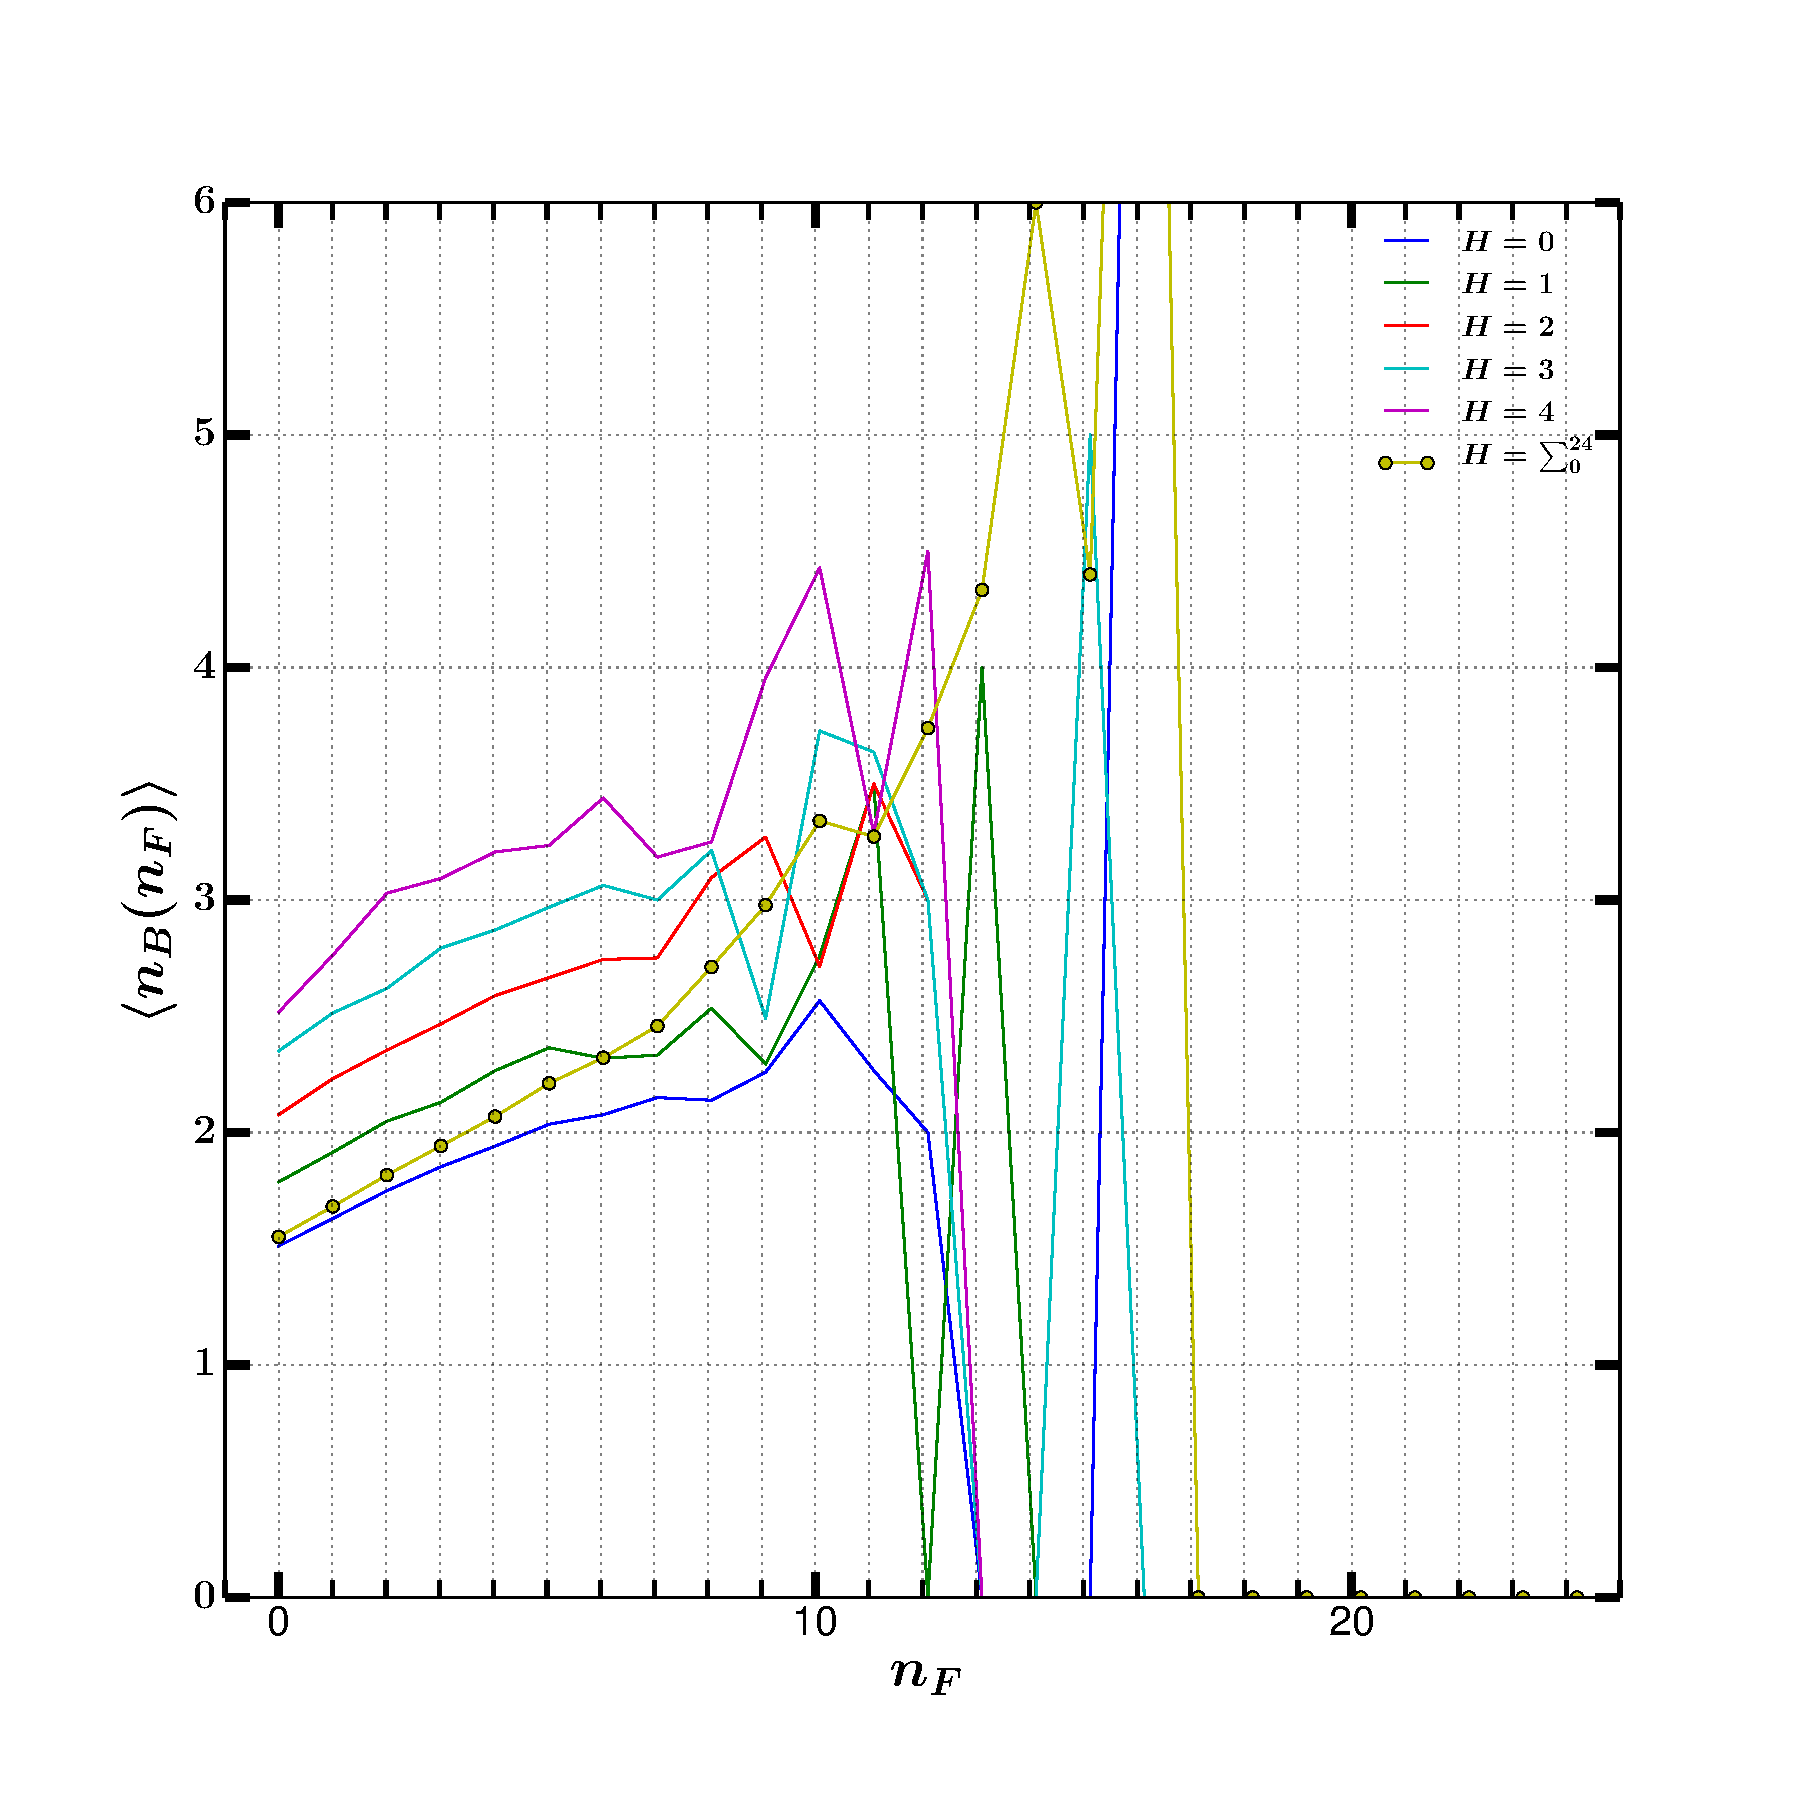
\includegraphics[scale=0.5]{../analyzed/nbnf_fixed_s_var_h.pdf}
    \caption[Fixed NPOMS and varying NPOMH]{}
\end{figure}

\newpage

\section*{\centering Non-Single diffraction, all diagrams except 1,4,6 and 10}

\subsubsection*{\centering N NPOMS and all NPOMH}
\begin{figure}[h!]
\centering
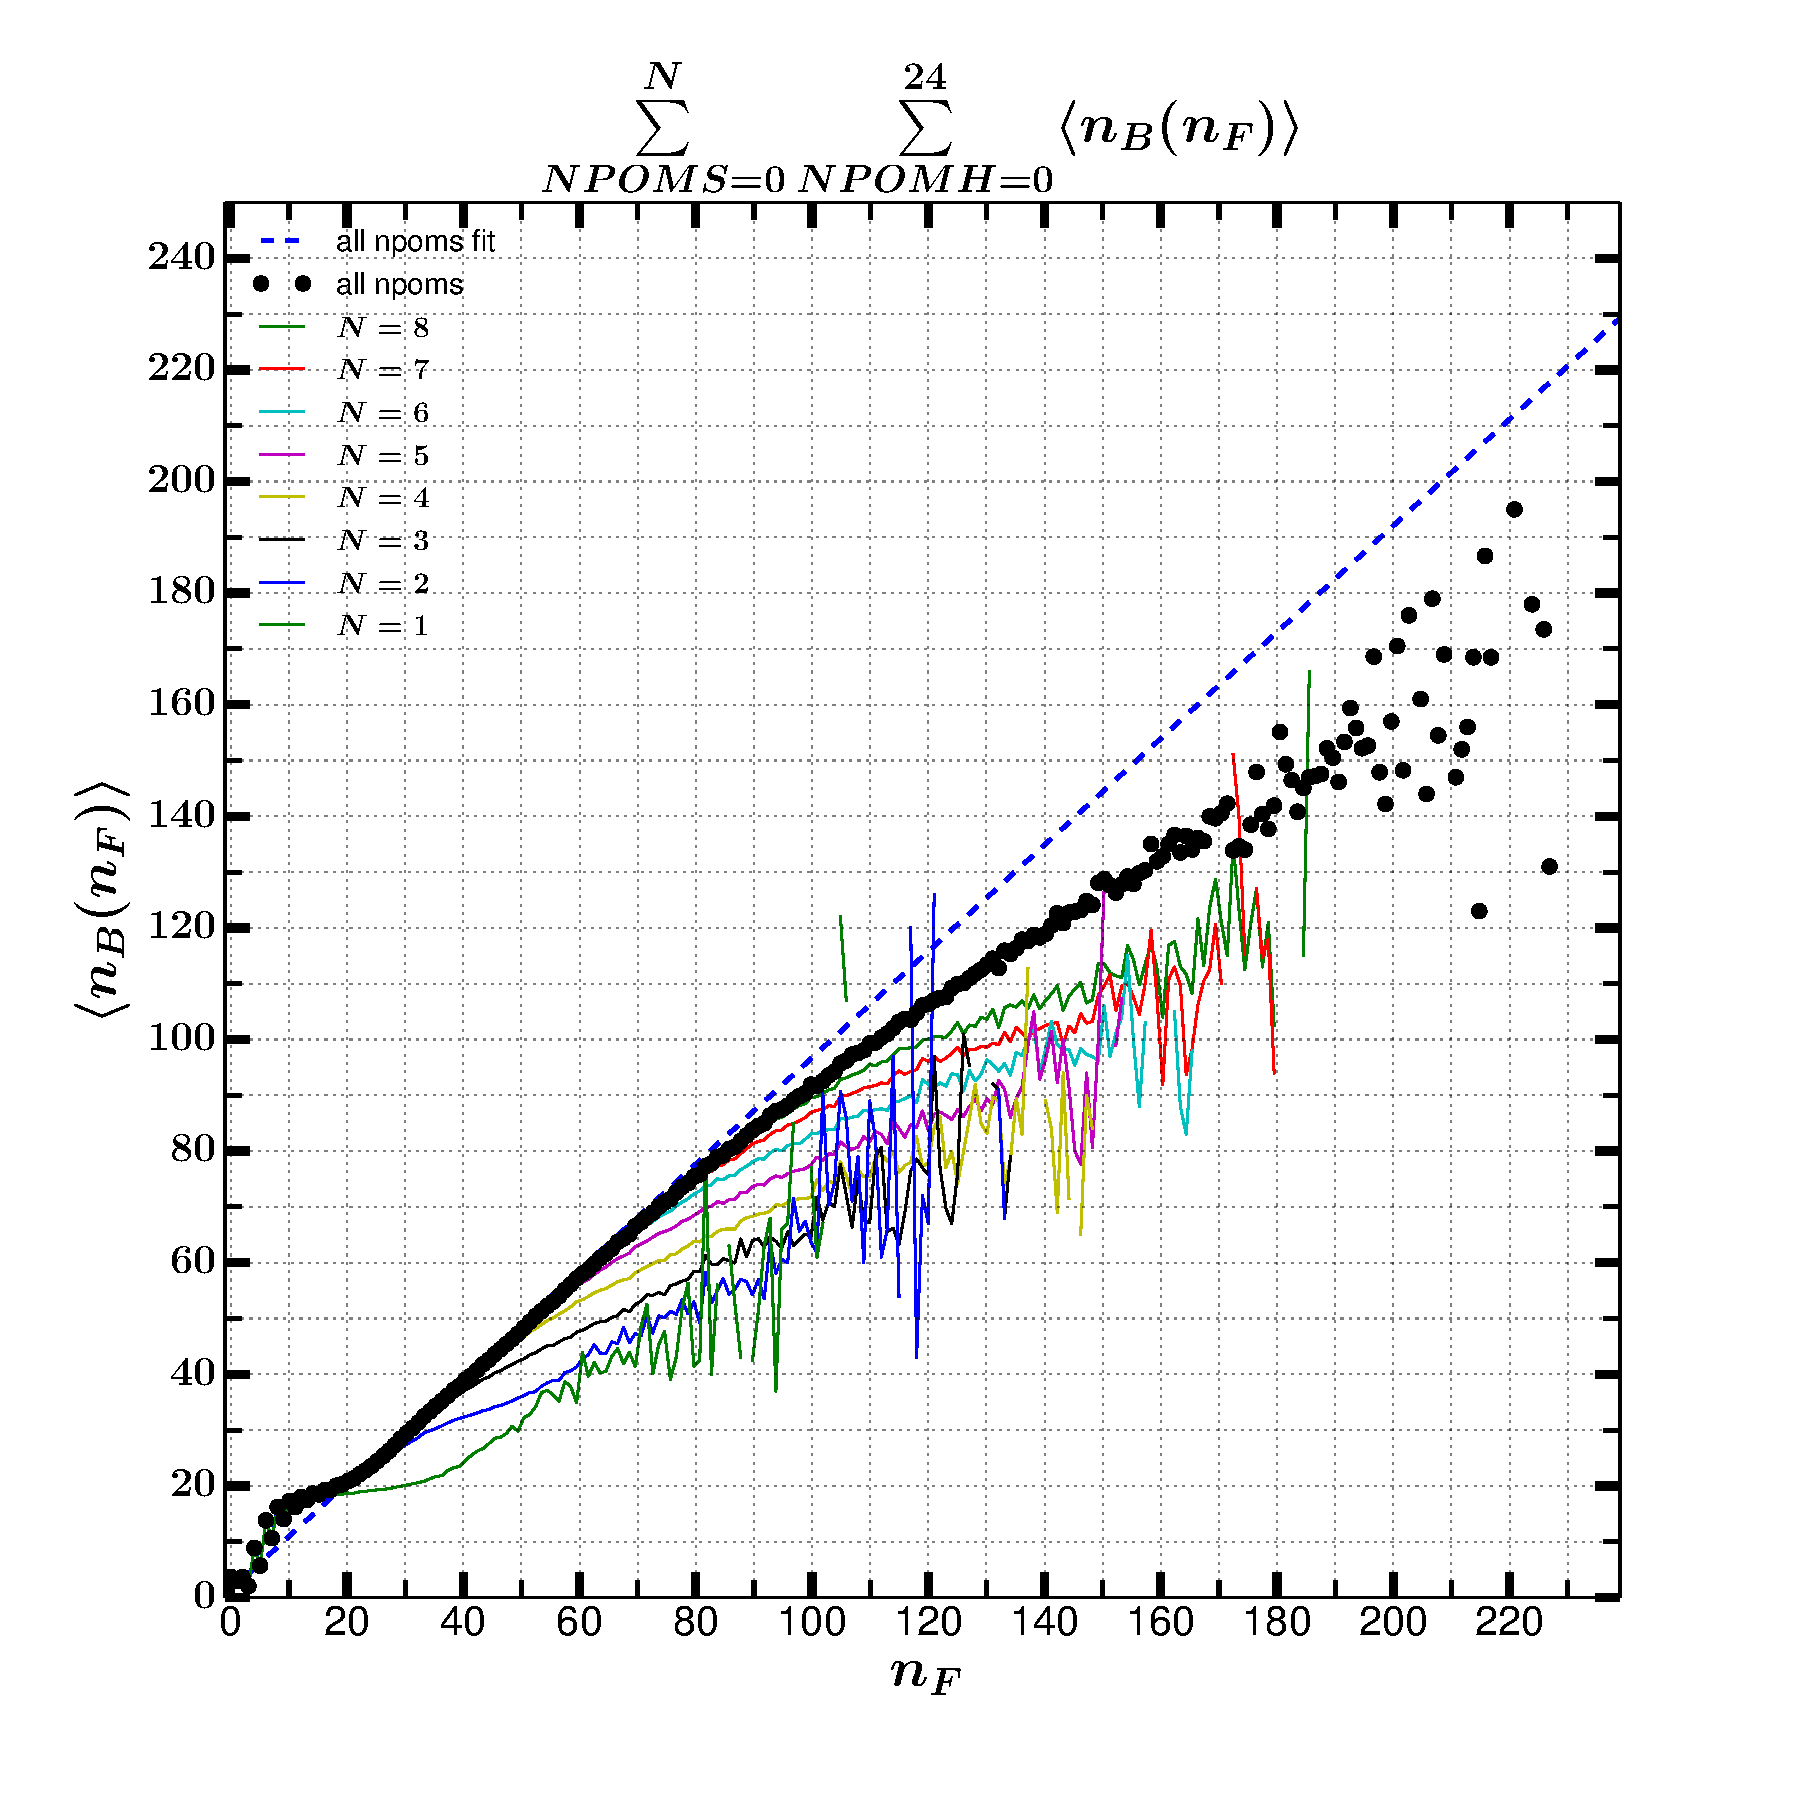
\includegraphics[scale=0.5]{../analyzed/nsd_nbnf_Nnpoms_allnpomh.pdf}
    \caption[NSD All NPOMS and NPOMH=0]{}
\end{figure}

\newpage
\subsubsection*{\centering All NPOMS and NPOMH=0}

\begin{figure}[h!]
    \centering
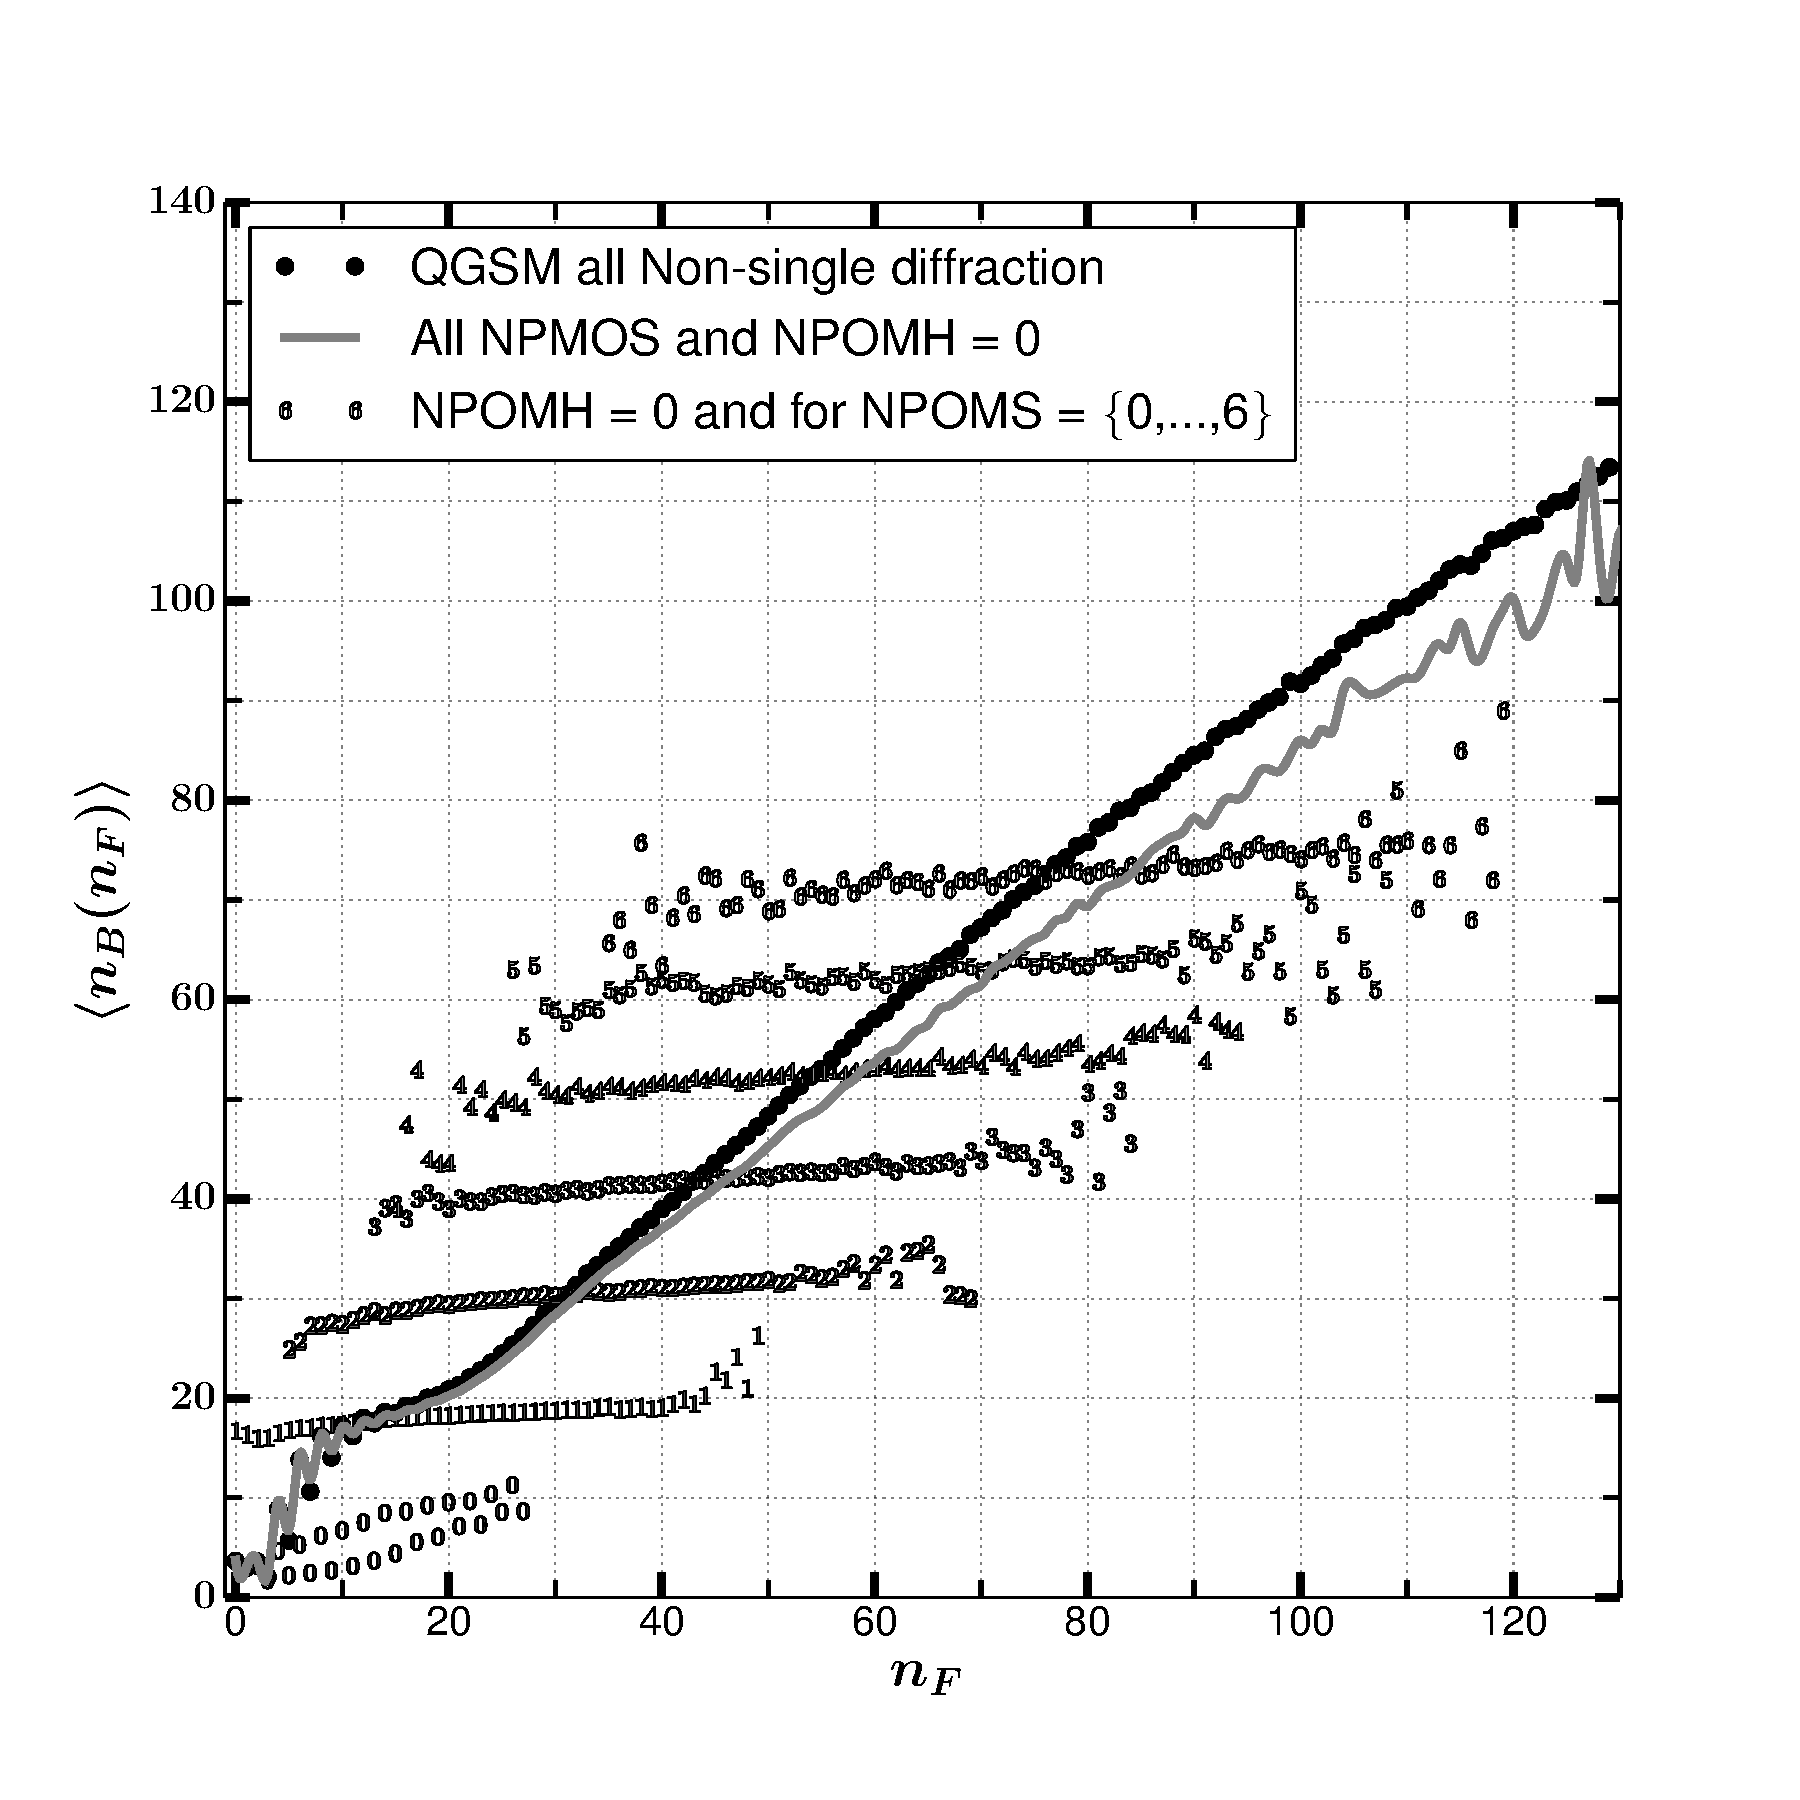
\includegraphics[scale=0.5]{../analyzed/nsd_nbnf_allnpoms_0npomh.pdf}
    \caption[NSD N NPOMS and all NPOMH]{}
\end{figure}

\newpage
\subsubsection*{\centering Fixed NPOMS and varying NPOMH}

\begin{figure}[h!]
    \centering
    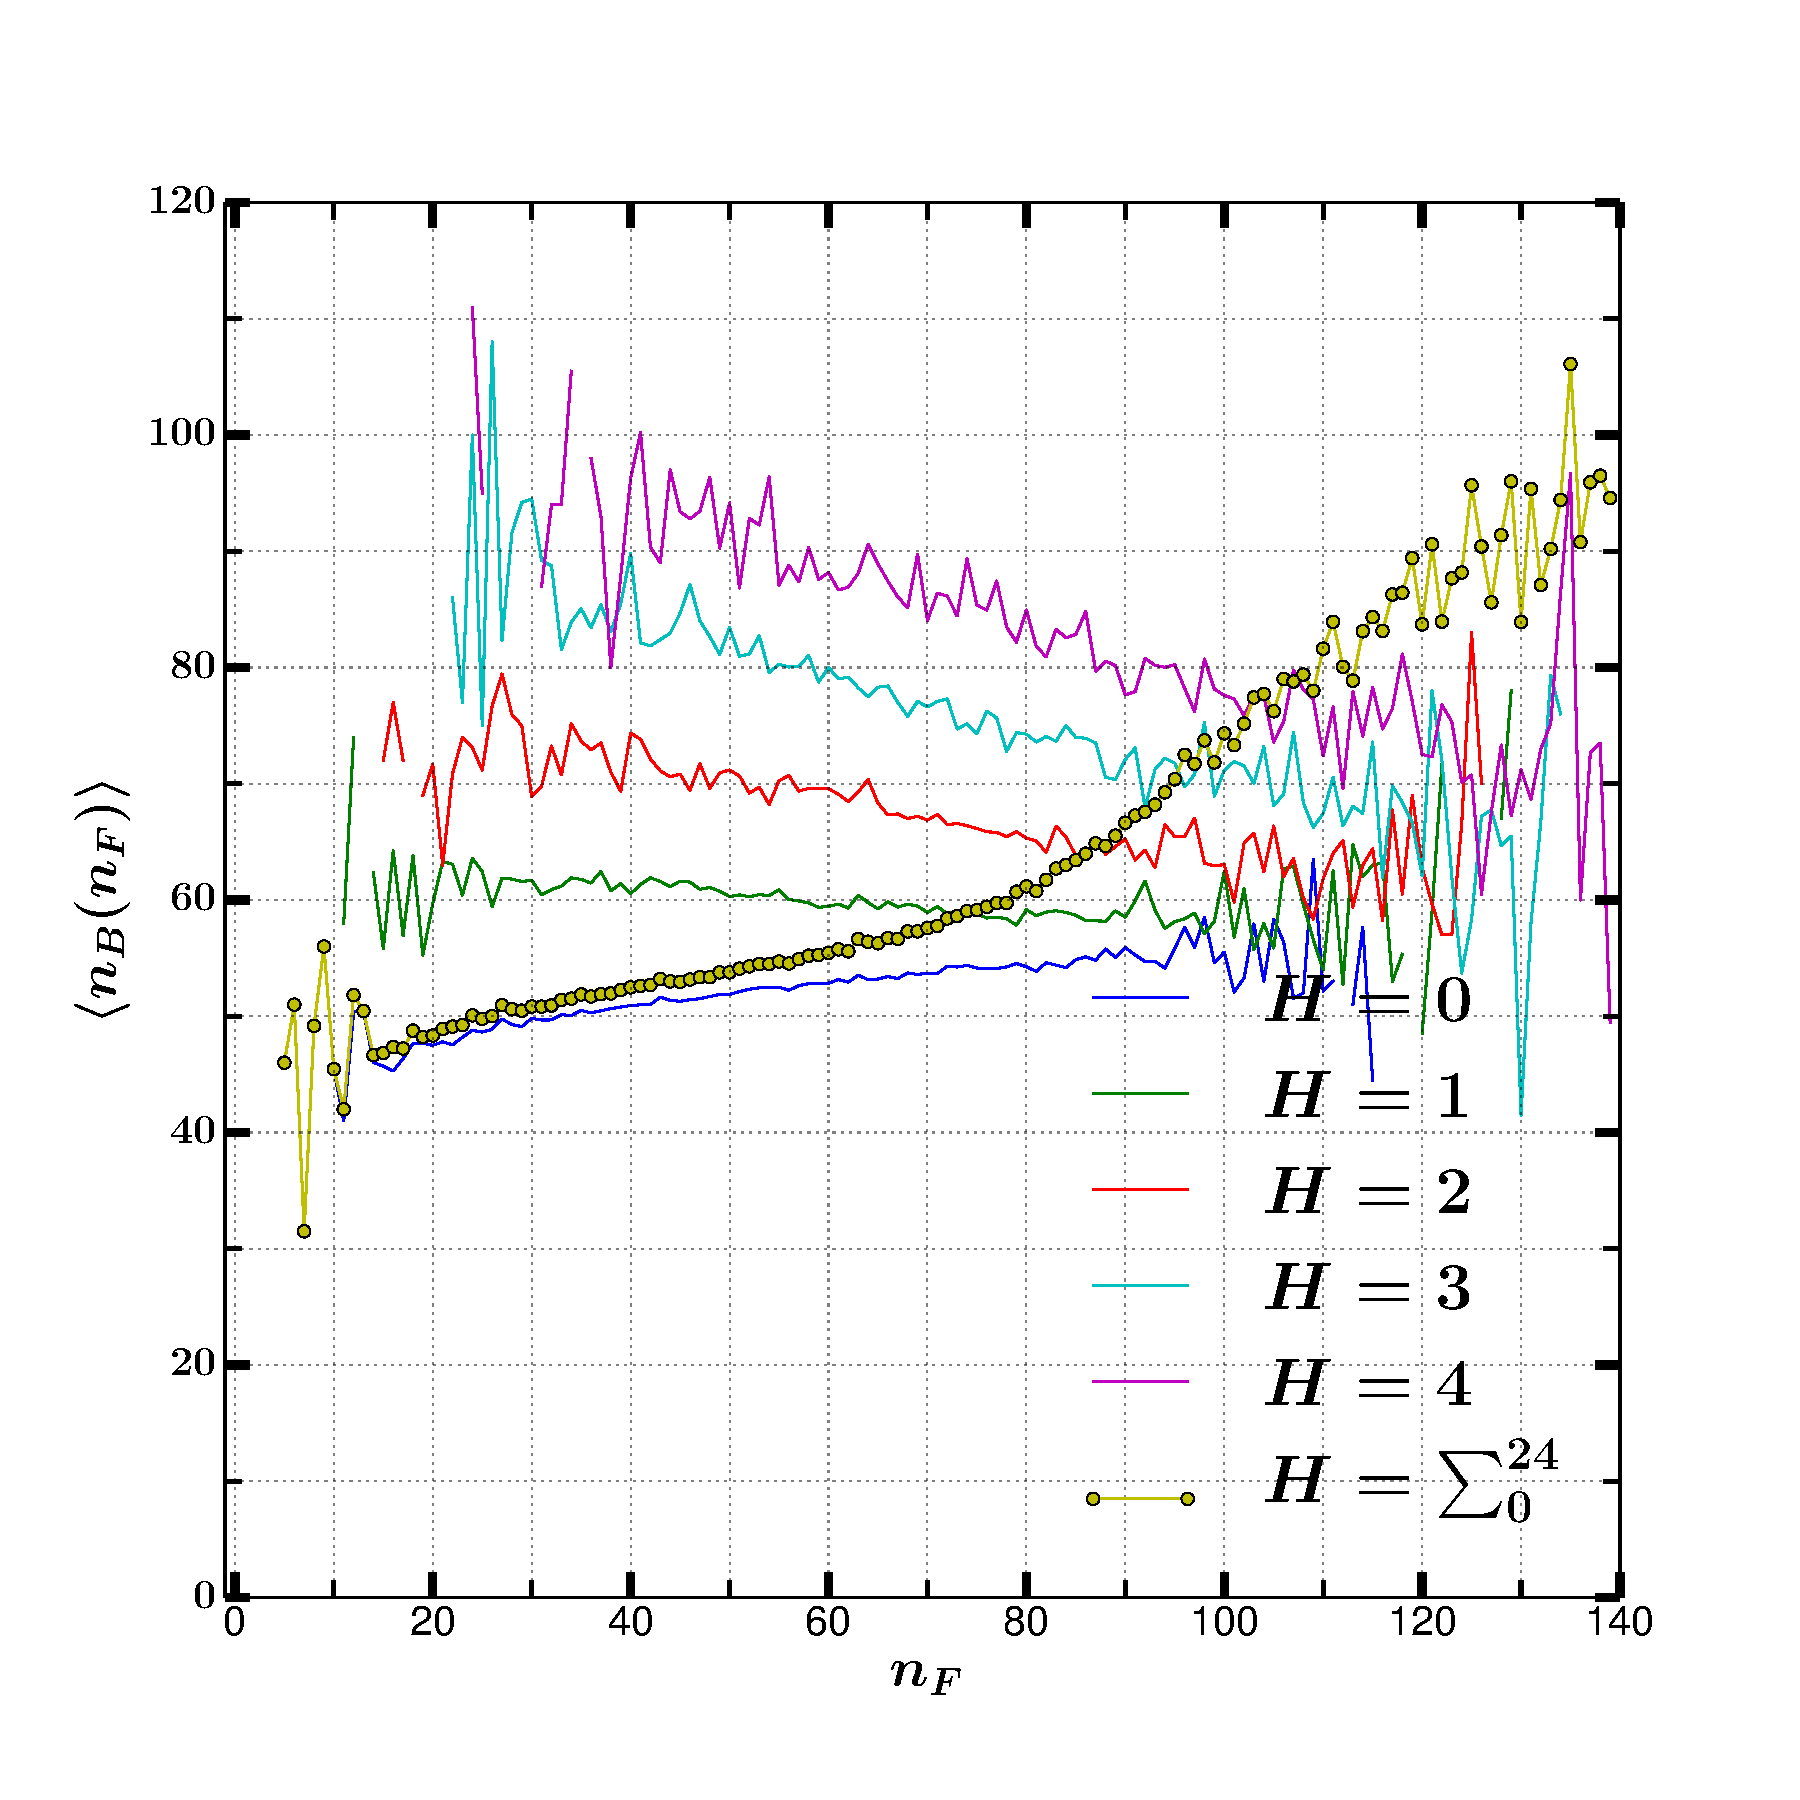
\includegraphics[scale=0.5]{../analyzed/nsd_nbnf_fixed_s_var_h.pdf}
    \caption[NSD Fixed NPOMS and varying NPOMH]{}
\end{figure}


\end{document}
